\documentclass[12pt]{article}
\usepackage{graphicx}
\usepackage[margin=25mm]{geometry}
\usepackage{amsmath}
\usepackage{amssymb}
\usepackage{biblatex}
\addbibresource{ref.bib}

\begin{document}

% Cover Page
\pagebreak

\begin{titlepage}
    \begin{center}
        \vspace*{\fill}
        Lab 1: The Scale Height of Earth's Atmosphere

        Author: Shaaz Feerasta

        CCID: feerasta

        Student ID: 1704756

        Lab Partner(s): Morgan Reinhart

        PHYS 126, LAB HR81

        TA: Nicolas Concha Marroquin

        Date of Lab: January 23, 2025
        \vspace*{\fill}
    \end{center}
\end{titlepage}
\vfill

\pagebreak

% Main Report
\section{Methods}

The data in this lab was collected using the pressure sensor on an iPhone 14 Pro, using the Phyphox app.
At each floor of the CCIS building at the University of Alberta North Campus, the phone was placed
and the pressure was recorded through the Phyphox app for approximately 10 seconds per floor.
After the 10 seconds was completed, the pressure recording was paused, and the phone was moved to a floor lower
and the process was repeated until we reached the bottom floor of the CCIS building.

From this process, approximately 100 data points were collected from a total of 7 floors.
Although we expected around 10 data points per floor, the data was not collected perfectly due to human error.

The reason we collected data from the CCIS building was because it is a tall building with many floors,
and primarily due to convenience. We chose approximately 10 seconds per floor also due to convenience and
the fact that 10 is a nice number to work with.

\section{Data}

\begin{figure}[h]
    \centering
    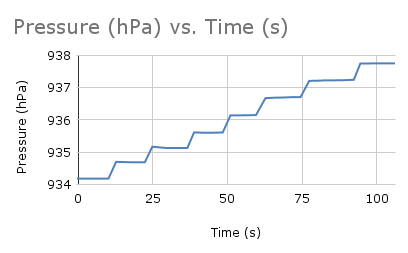
\includegraphics[width=0.8\textwidth]{Pressure-Time.png}
    \caption{Displays a line graph of the pressure data collected from different floors of the CCIS building
    at the University of Alberta North Campus in Pascals, plotted against time in seconds. Each jump in the graph represents a
    transition to a different floor.}
    \label{fig:pressure-time}
\end{figure}

\section{Analysis}

As explained above, the data itself was collected using an iPhone 14 Pro pressure sensor,
along with the Phyphox app. The data itself was collected in hector Pascals (hPa), and was
plotted against time in seconds. The data was collected from the CCIS building at the University of Alberta North Campus,
where the pressure was recorded at each of the 7 floors of the building. There were no repeated measurements required,
however; if needed, we would let the phone sit for a longer time in order to average out the data, or simply repeat the entire experiment since
it is at a smaller scale.

Further, the data was converted from hPa to Pa, and then averaged using altitude rather than timestamps for the remainder of the calculations.

When analyzing the data and finding the slope, we decided to use the average of the data points of each floor rather than the entirety of the dataset.
This was done to simplify the data and make it easier to work with. As an alternative, we could have assigned a height value to each data point and
analyzed from that point onwards. The differences would have been negligible.

\section{Analysis Plot}
\begin{figure}[h]
    \centering
    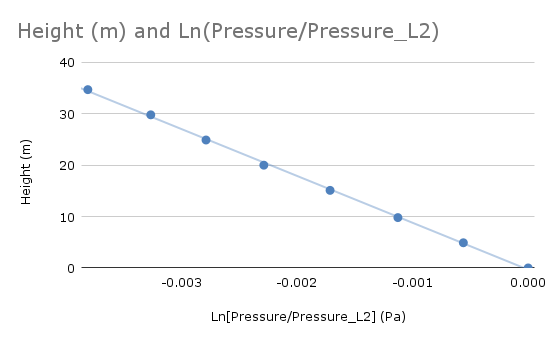
\includegraphics[width=0.8\textwidth]{Height-LogData.png}
    \caption{Displays a scatter plot of the natural logarithm of the pressure data ratio collected from different floors of the CCIS building.
    The line fits the equation $z = -H\ln\frac{P}{P_{L2}} + 0$.
    $z$ is our height in metres, $H$ is the scale height of Earth's atmosphere, 
    $P$ ($\pm 0.05$ Pa) is the pressure at the floor at height $z$,
    and $P_{L2}$ ($\pm 0.05$ Pa) is the pressure at the lowest floor.
    Using LINEST, we get that $-H = (-9.1 \pm 0.1) \times 10^3 \, \mathrm{m}$,
    and intercept $b = (-3 \pm 2) \times 10^{-1}\, \mathrm{m}$.}
\end{figure}

\section{Calculation}
Based on our LINEST slope and intercept, 
\begin{align*}
    -H &= (-9.1 \pm 0.1) \times 10^3 \, \mathrm{m} \\
    \therefore H &= (9.1 \pm 0.1) \times 10^3 \, \mathrm{m} \\
    -b &= (-3 \pm 2) \times 10^{-1}\, \mathrm{m} \\
    \therefore b &=(3 \pm 2) \times 10^{-1}\, \mathrm{m}
\end{align*}

Compared to our theoretical value for the scale height of Earth's atmosphere, $H_{theoretical} = 8.4 \, \mathrm{km} = 8.4 \times 10^3\, \mathrm{m}$,
our experimental value of $H$ is greater than three error intervals away from our experimental value,
i.e. $H_{theoretical} >3 \delta H$.
However, our experimental value of $b$ is within two error intervals of the theoretical value of $b = 0$.
This may be due to a data collection error, or simply just a varying result from a purely theoretical value.

\begin{thebibliography}{9}

    \bibitem{labmanual} 
    Department of Physics. \textit{PHYS 126 Lab Manual}. University of Alberta, 2025.

    \bibitem{person}
    TA assisted with the lab, and provided guidance on the data collection and analysis.

    \bibitem{person}
    Lab partner Morgan Reinhart assisted with the data collection and analysis.
    
    \end{thebibliography}
\end{document}